\documentclass[aspectratio=169]{beamer}
\usetheme{Madrid}
\usecolortheme{dolphin}

\usepackage[utf8]{inputenc}
\usepackage{lmodern}
\usepackage{amsmath,amssymb}
\usepackage{tikz}
\usetikzlibrary{arrows.meta,positioning,shapes.geometric,decorations.pathreplacing}
\usepackage{listings}
\usepackage{xcolor}
\usepackage{booktabs}
\usepackage{array}

\setbeamertemplate{navigation symbols}{}
\setbeamertemplate{footline}[frame number]

\definecolor{reserveorange}{RGB}{224,123,57}
\definecolor{mainblue}{RGB}{44,110,158}
\definecolor{codebg}{RGB}{244,244,244}

\lstset{
  basicstyle=\ttfamily\scriptsize,
  backgroundcolor=\color{codebg},
  frame=single,
  breaklines=true,
  columns=fullflexible,
  keywordstyle=\color{mainblue}\bfseries,
  commentstyle=\color{gray}\itshape,
  language=Python,
}

% ---- RESERVE slide marker: colored corner badge, drawn on every reserve slide ----
\newcommand{\reservebadge}{%
  \begin{tikzpicture}[remember picture, overlay]
    \node[anchor=north east, xshift=-0.15cm, yshift=-0.05cm,
          fill=reserveorange, text=white, font=\bfseries\small,
          rounded corners=2pt, inner sep=4pt]
      at (current page.north east) {RESERVE};
  \end{tikzpicture}%
}

\title{Pinhole Aperture Optics for Myopia Correction}
\subtitle{Theory, Simulation, and Photographic Validation of a Reduced-Eye Diffraction/Defocus Model}
\author{IYPT Team}
\date{2026}

\begin{document}

% ============================================================ TITLE
\begin{frame}
  \titlepage
\end{frame}

% ============================================================ AGENDA
\begin{frame}{Presentation Roadmap}
  \begin{block}{Part 1 (this deck)}
    Introduction \quad$\to$\quad Theoretical Model \quad$\to$\quad Evaluators/Metrics Overview
  \end{block}
  \vspace{0.3cm}
  \begin{block}{Later parts (not in this deck)}
    Experiment 1 (ExP2 photographic validation) \quad$\to$\quad Experiment 2 (ExP3 optical bench)
    \quad$\to$\quad Array design \& fabrication \quad$\to$\quad Discussion
  \end{block}
  \vspace{0.5cm}
  \begin{alertblock}{How this deck is organized}
    Every slide from the main talk is followed, where relevant, by \textcolor{reserveorange}{\textbf{RESERVE}}
    slides carrying the full derivation, code, or extended data. Nothing is cut --
    reserve slides exist for defending any question in depth during the jury discussion.
  \end{alertblock}
\end{frame}

% ============================================================================
\section{Introduction}
% ============================================================================

\begin{frame}{Section 1: Introduction}
  \tableofcontents[currentsection]
\end{frame}

\begin{frame}{The Problem: Correcting Myopia Without a Lens}
  \begin{columns}
    \begin{column}{0.55\textwidth}
      \begin{itemize}
        \item A myopic (short-sighted) eye focuses distant light \textbf{in front of}
          the retina, not on it -- the retinal image is a blur disc, not a point.
        \item Standard correction: a diverging lens (glasses/contacts) restores focus.
        \item \textbf{Pinhole optics} offer a lens-free alternative: a small aperture
          placed in front of the eye restricts the cone of rays reaching the retina,
          shrinking the blur disc geometrically -- \emph{without} refracting light at all.
        \item This is the physical basis of pinhole glasses, marketed as a
          correction-free vision aid.
      \end{itemize}
    \end{column}
    \begin{column}{0.45\textwidth}
      \centering
      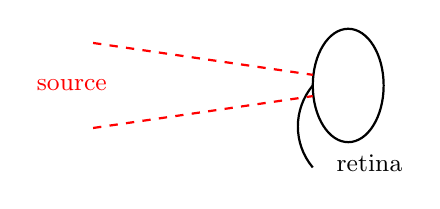
\begin{tikzpicture}[scale=0.9]
        % eye
        \draw[thick] (2.6,0) ellipse (0.5 and 0.8);
        \draw[thick] (2.1,0) arc (140:220:0.9);
        % blurred cone without pinhole (dashed, wide)
        \draw[dashed, red, thick] (-1,0.6) -- (2.1,0.15);
        \draw[dashed, red, thick] (-1,-0.6) -- (2.1,-0.15);
        \node[red] at (-1.3,0) {\small source};
        \node at (2.9,-1.1) {\small retina};
      \end{tikzpicture}
      \vspace{0.2cm}
      \small A myopic eye: the marginal rays (dashed) converge in front of the
      retina, spreading into a blur circle at the retinal plane.
    \end{column}
  \end{columns}
\end{frame}

\begin{frame}{Why This Is a Genuine Physics Problem, Not Just Engineering}
  \begin{itemize}
    \item Shrinking the aperture reduces \textbf{geometric} blur linearly with
      aperture diameter -- naively, smaller is always better.
    \item But a small aperture increases \textbf{diffraction} blur
      (Airy-disk scale $\propto 1/a_{\text{hole}}$) -- naively, larger is always better.
    \item These two effects trade off oppositely with aperture size $\Rightarrow$
      there is an \textbf{optimum aperture} for every myopic power $M$, not a
      "smaller is always better" answer.
    \item This project's core question: \emph{find that optimum, validate it
      against real photographic measurement, and check it against independent
      clinical literature.}
  \end{itemize}
  \vspace{0.3cm}
  \begin{alertblock}{This is exactly the geometric/diffraction competition this
    project's full theoretical model (Section 2) is built to resolve quantitatively.}
  \end{alertblock}
\end{frame}

\begin{frame}{Project Scope -- What Was Actually Built and Tested}
  \begin{columns}
    \begin{column}{0.5\textwidth}
      \textbf{Theory}
      \begin{itemize}
        \item Full wave-optics (Angular Spectrum Method) simulation
        \item Closed-form RSS approximation, cross-checked against it
        \item Two-pinhole ghost-image separation formula (validated, $R^2=0.995$)
        \item Gaze-weighted safety/comfort evaluation
      \end{itemize}
      \textbf{Experiment}
      \begin{itemize}
        \item ExP2: real point-source photography, 5 apertures, phone camera
        \item ExP3: independent frosted-screen optical-bench sweep, 6 apertures
      \end{itemize}
    \end{column}
    \begin{column}{0.5\textwidth}
      \textbf{Cross-checks}
      \begin{itemize}
        \item Clinical literature anchor (Miller \& Johnson 1977, via Shen 2026)
        \item No-reference image-quality scoring (BRISQUE) on real scene photos
      \end{itemize}
      \textbf{Design output}
      \begin{itemize}
        \item Gaze-weighted multi-pinhole array design, per myopic power $M$
        \item A real photochemical-etching fabrication specification (0.05mm brass
          shim, UV photoresist)
      \end{itemize}
    \end{column}
  \end{columns}
  \vspace{0.2cm}
  \small\textit{This deck's Part 1 covers Introduction + Theoretical Model only.}
\end{frame}

\begin{frame}{Research Questions}
  \begin{enumerate}
    \item What is the theoretically optimal pinhole aperture at each myopic
      power $M$, once diffraction is modeled properly (not just geometric optics)?
    \item Does a real photographic measurement of blur growth with $M$ match
      that theory -- and if not, where and why?
    \item Does a simpler closed-form approximation (RSS) do just as well as
      the full wave-optics simulation, or is the extra complexity justified?
    \item Does this project's own theoretical aperture-tolerance prediction
      agree with independent clinical literature?
    \item Can a \emph{multi-pinhole array} (rather than one hole) be designed
      that stays ghost-free across natural gaze movement, and can it actually
      be fabricated?
  \end{enumerate}
\end{frame}

% ============================================================================
\section{Theoretical Model}
% ============================================================================

\begin{frame}{Section 2: Theoretical Model}
  \tableofcontents[currentsection]
\end{frame}

\begin{frame}{2.1 The Reduced-Eye Model}
  \begin{itemize}
    \item Every theoretical prediction in this project uses a single-surface
      \textbf{reduced eye}: a thin lens of fixed power $P_0$, immersed on its
      image side in vitreous of refractive index $n'$.
    \item Myopic defocus is modeled as an \textbf{added power} $M$ (diopters)
      at the eye/lens -- exactly as an induced-refractive-error lens would.
    \item Image-side (media-reduced) focal length:
  \end{itemize}
  \[
    f'_{\text{image}} = \frac{n'}{P_0}
  \]
  \begin{alertblock}{Not the naive $f'=1/P_0$}
    That simpler form is only correct if image space were air. This project's
    own source code uses \texttt{refractive\_index\_correction=True} throughout,
    so $n'$ must appear.
  \end{alertblock}
  \textbf{Constants used everywhere in this project (traced to source, not assumed):}
  \[
    P_0 = 60.0\ \text{D}, \qquad n' = 1.336, \qquad \lambda_{\text{vacuum}} = 550\ \text{nm}
  \]
  {\scriptsize $\Rightarrow f'_{\text{image}} = \dfrac{1.336}{60.0}\times10^6\ \mu\text{m} = 22266.667\ \mu\text{m}$}
\end{frame}

\begin{frame}{2.2 The Blur Metric: Encircled-Energy Radius $r_{EE50}$}
  \begin{itemize}
    \item Every model and every measurement in this project reduces to one
      number per (aperture, defocus) condition: the radius that encloses 50\%
      of the total collected optical energy.
    \item Chosen because it is well-defined for \emph{both} a simulated
      point-spread function \emph{and} a real, noisy photograph of a point
      source -- unlike a fitted Gaussian $\sigma$, which assumes a shape the
      real data may not follow.
  \end{itemize}
  \[
    \sum_{r_i \leq r_{EE50}} I(r_i) \;=\; 0.5 \times \sum_{i} I(r_i)
  \]
  \begin{block}{Used identically in three places}
    \begin{itemize}
      \item ASM simulation table (physical $\mu$m, from the retinal irradiance map)
      \item ExP2 photographic pipeline (pixels, background-subtracted blob)
      \item RSS closed-form estimate (physical $\mu$m, analytic)
    \end{itemize}
  \end{block}
\end{frame}

\begin{frame}{2.3 Model A -- Full Wave-Optics Simulation (ASM)}
  \begin{columns}
    \begin{column}{0.55\textwidth}
      \begin{itemize}
        \item The primary theoretical prediction is \textbf{not} an analytic
          formula -- it is a full scalar-diffraction simulation: the
          \textbf{Angular Spectrum Method}.
        \item Propagates a coherent field from the aperture, through a 12mm
          air gap, through the eye lens (adding power $P_0+M$ as a quadratic
          phase), to the retina.
        \item Run once, from scratch, across a grid of 15 aperture sizes
          $\times$ 8 myopic powers $M$ (120 points) $\to$ the single theory
          table (\texttt{blur\_sweep.csv}) every comparison in this project uses.
      \end{itemize}
    \end{column}
    \begin{column}{0.45\textwidth}
      \centering
      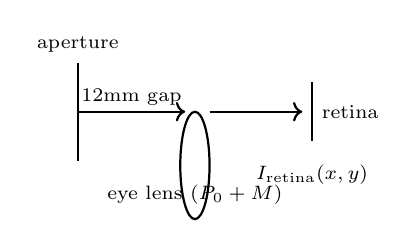
\begin{tikzpicture}[scale=0.62, every node/.style={font=\scriptsize}]
        \draw[thick] (0,-1) -- (0,1) node[above]{aperture};
        \draw[->, thick] (0,0) -- (2.2,0);
        \node at (1.1,0.3) {12mm gap};
        \draw[thick] (2.4,-1.1) ellipse (0.3 and 1.1);
        \node[below] at (2.4,-1.3) {eye lens $(P_0+M)$};
        \draw[->, thick] (2.7,0) -- (4.6,0);
        \draw[thick] (4.8,-0.6) -- (4.8,0.6);
        \node[right] at (4.8,0) {retina};
        \node[below] at (4.8,-0.9) {$I_{\text{retina}}(x,y)$};
      \end{tikzpicture}
    \end{column}
  \end{columns}
  \vspace{0.2cm}
  \small Grid: 4096$\times$4096, 6mm window (dx $\approx1.465\,\mu$m/px) --
  this exact pixel size later sets the measurement-uncertainty floor used in
  the ghost-margin safety framework.
\end{frame}

\begin{frame}{2.4 Model B -- Closed-Form Approximation (RSS)}
  \begin{itemize}
    \item ASM is expensive (a full 4096$\times$4096 propagation per point) and
      opaque as a design tool. RSS combines geometric and diffraction blur in
      quadrature -- a much faster, simpler estimator, checked independently
      against the same measured photographs ASM is checked against.
  \end{itemize}
  \[
    c_{\text{geom}}(a,M) = \frac{a\cdot M}{P_0}
    \qquad\qquad
    c_{\text{diff}}(a) = 1.22\,\frac{\lambda_{\text{eff}}\,f'}{a}
  \]
  \[
    c_{\text{RSS}}(a,M) = \sqrt{c_{\text{geom}}(a,M)^2 + c_{\text{diff}}(a)^2}
  \]
  \begin{alertblock}{Headline result (full data in Results deck, not here)}
    ASM matches the measured photographs decisively better than RSS across
    every comparable case (18/18 rows). RSS is kept because it is the
    \emph{only} model computable with no measured/simulated $M=0$ reference --
    useful, but not the primary predictive model.
  \end{alertblock}
\end{frame}

\begin{frame}{2.5 Model C -- Two-Pinhole Ghost-Image Separation}
  \begin{itemize}
    \item For a multi-pinhole \textbf{array} design: two neighboring holes each
      form their own retinal image of a point source. Under defocus, these
      separate spatially -- a visible "ghost" once the separation exceeds the
      eye's own resolvable blur.
  \end{itemize}
  \[
    \Delta r(s,M) = \frac{s\cdot M}{P_0 - M}
  \]
  \begin{block}{Independently validated}
    $R^2=0.995$ against a separate two-hole coherent wave-optics simulation
    (32 points), vs. $R^2=-1701.71$ for an earlier, disproven formula.
  \end{block}
  This formula, combined with a safety-margin framework (Section 2.7), is
  what makes a physically buildable \emph{array} design possible, not just a
  single optimal hole.
\end{frame}

\begin{frame}{2.6 Evaluators / Metrics -- What This Project Actually Measures}
  \small
  \begin{tabular}{@{}p{3.6cm}p{8.7cm}@{}}
    \toprule
    \textbf{Evaluator} & \textbf{What it quantifies} \\
    \midrule
    $r_{EE50}$ & Blur radius -- primary metric, theory \emph{and} both experiments \\
    RSS vs.\ ASM \% deviation & Which theoretical model actually fits measured data \\
    Ghost margin (worst-case) & Hard safety gate: is a design ghost-free at \emph{every} tested gaze angle \\
    Gaze-weighted ghost/blind \% & Realistic-use metric: \% of actual viewing \emph{time} spent ghosting/blind, using measured eye-tracking eccentricity data \\
    LogMAR / acuity-optimal aperture & Clinical-acuity-based optimum, cross-checked against the pure-blur optimum \\
    BRISQUE (no-reference IQA) & Real-scene photo quality score, independent of the point-source pipeline \\
    \bottomrule
  \end{tabular}
  \vspace{0.3cm}
  \begin{alertblock}{Why so many evaluators, not just one}
    Worst-case and gaze-weighted answer \emph{different} questions (hard
    guarantee vs.\ realistic experience) -- this project reports both,
    deliberately, rather than picking one and hiding the other.
  \end{alertblock}
\end{frame}

\begin{frame}{2.7 Safety-Margin Framework (Why a Margin, Not Just a Sign)}
  \begin{itemize}
    \item A design "passes" only if its margin clears a \textbf{known, sourced
      uncertainty} in the underlying measurement -- not merely margin $>0$.
  \end{itemize}
  \[
    \text{margin} = 1 - \frac{\Delta r_{\text{actual}}}{r_{\text{resolvable}}},
    \qquad
    \text{threshold} = \frac{2.0\times \delta_{r,\text{unc}}}{r_{\text{resolvable}}}
  \]
  \[
    \delta_{r,\text{unc}} = 2\times dx_{\text{grid}} = 2\times1.465\,\mu\text{m} = 2.93\,\mu\text{m}
  \]
  \begin{block}{Audit history, reported honestly (full trail in Reserve)}
    An earlier version of this framework required only margin $>0$ -- found to
    silently reward a design with \emph{zero illuminated holes} (infinite
    margin, zero usefulness). Fixed by adding an independent viability gate.
  \end{block}
\end{frame}

\begin{frame}{Section 2 Summary -- What Carries Into the Rest of the Talk}
  \begin{itemize}
    \item One consistent eye model ($P_0=60$D, $n'=1.336$) feeds every
      theoretical number in this project -- no separately invented constants.
    \item Two independent theoretical models (ASM, RSS) exist so the
      photographic experiments (Part 2) test \emph{model choice}, not just
      \emph{model fit}.
    \item The ghost-separation formula and safety-margin framework
      (Section 2.5/2.7) are what let this project go from "one optimal hole"
      to "a real, checkable multi-pinhole array design" (Part 3).
    \item Every evaluator above will reappear with real numbers in the
      Results parts of this talk.
  \end{itemize}
  \vspace{0.3cm}
  \centering\Large Next: Experiment 1 -- Photographic Validation (Part 2, separate deck)
\end{frame}

% ============================================================================
% ============================ RESERVE / BACKUP SECTION ======================
% ============================================================================
\section*{Reserve Slides}
\begin{frame}
  \reservebadge
  \centering
  \vspace{2cm}
  {\Huge\bfseries\textcolor{reserveorange}{RESERVE SLIDES}}\\[0.5cm]
  {\large Full derivations, source code, and extended data for every model
  and evaluator in Section 2.}\\[0.3cm]
  \small Not part of the timed talk -- called up during jury Q\&A as needed.
\end{frame}

\begin{frame}{R1 -- ASM: Full Simulation Pipeline}
  \reservebadge
  \begin{enumerate}
    \item Circular aperture radius $a_{\text{hole}}$ illuminated by a coherent
      plane wave, $\lambda=550$nm vacuum.
    \item Angular-spectrum free-space propagation, 12mm gap, on a
      4096$\times$4096 grid spanning a 6mm window
      ($dx = 6000/4096 \approx 1.465\,\mu$m/pixel).
    \item Eye/lens applies a quadratic phase for total power $(P_0+M)$, using
      the reduced, media-corrected convention.
    \item Propagate the eye's own image-side focal distance $f'$ to the
      retina $\Rightarrow$ irradiance map $I_{\text{retina}}(x,y)$.
    \item $r_{EE50/70/80/90}$ and RMS spot radius computed by radial
      integration of $I_{\text{retina}}$.
  \end{enumerate}
  \textbf{Grid history (reported honestly):} an earlier run used a
  2048-point grid; found to give $r_{EE50}$ values exactly $2\times$ too
  large for large apertures (a known grid-resolution artifact). Fixed to
  4096; the stale file was preserved, not deleted
  (\texttt{blur\_sweep\_gridN2048\_legacy.csv}).
\end{frame}

\begin{frame}[fragile]{R1b -- ASM Sweep: Source Code}
  \reservebadge
  \begin{lstlisting}
result = p2.run_pipeline_point(
    a_hole=a_um * 1e-6, wavelength=WAVELENGTH_NM * 1e-9,
    d_gap=D_GAP_MM * 1e-3, grid_N=GRID_N, window_L_mm=WINDOW_L_MM,
    M_diopters=M, P0=60.0, n_prime=1.336,
    D_pupil_um=D_PUPIL_UM, refractive_index_correction=True,
)
if result["junction_check_passed"]:
    I_retina = result["I_retina"]
    dx = result["cornea_result"]["dx"]
    r_edges, EE, total_power = junction.encircled_energy(I_retina, R, dx)
    for p in PERCENTILES:
        row[f"r_EE_{int(p*100)}_um"] = junction.r_for_EE(r_edges, EE, p) * 1e6
  \end{lstlisting}
  \small \texttt{new\_sweeps/run\_blur\_sweep.py} -- generates
  \texttt{blur\_sweep.csv}, the single theory source table for this entire
  project.
\end{frame}

\begin{frame}{R2 -- RSS: Full Derivation}
  \reservebadge
  \textbf{Geometric defocus term} -- a defocus of $M$ diopters, with total eye
  power $P_0$, produces a ray-optics blur circle scaling linearly with
  aperture radius and $M$ relative to $P_0$:
  \[
    c_{\text{geom}}(a,M) = \frac{a\cdot M}{P_0}
  \]
  \textbf{Diffraction term} -- Airy-disk-scale blur at the retina, using the
  \emph{effective (media-reduced)} wavelength, not the raw vacuum value:
  \[
    c_{\text{diff}}(a) = 1.22\,\frac{\lambda_{\text{eff}}\,f'}{a},
    \qquad
    \lambda_{\text{eff}} = \frac{\lambda_{\text{vacuum}}}{n'} = \frac{0.550}{1.336}\,\mu\text{m} = 0.4117\,\mu\text{m}
  \]
  \begin{alertblock}{Why the media-reduced wavelength}
    Pairing the media-reduced $f'=n'/P_0$ with the raw vacuum wavelength would
    under-apply the lens's converging phase by a factor of $n'$ -- this
    project's own source module explicitly warns against exactly that
    inconsistency.
  \end{alertblock}
  Normalization: at $M=0$, $c_{\text{geom}}=0$ identically, so
  $c_{\text{RSS}}(a,0)=c_{\text{diff}}(a)$ alone -- the only model needing no
  measured/simulated $M=0$ reference at all.
\end{frame}

\begin{frame}[fragile]{R2b -- RSS: Source Code}
  \reservebadge
  \begin{lstlisting}
P0 = 60.0
N_PRIME = 1.336
LAMBDA_VACUUM_UM = 550.0 / 1000.0
LAMBDA_UM = LAMBDA_VACUUM_UM / N_PRIME   # media-reduced
F_PRIME_UM = (N_PRIME / P0) * 1e6

def c_geom_um(a_hole_um, M):
    return a_hole_um * M / P0

def c_diff_um(a_hole_um):
    return 1.22 * LAMBDA_UM * F_PRIME_UM / a_hole_um

def c_tot_rss_um(a_hole_um, M):
    return math.sqrt(c_geom_um(a_hole_um, M)**2 + c_diff_um(a_hole_um)**2)

def predicted_ratio_rss(a_hole_um, M):
    return c_tot_rss_um(a_hole_um, M) / c_tot_rss_um(a_hole_um, 0.0)
  \end{lstlisting}
  \small \texttt{ExperimentalComparison/rss\_comparison.py}
\end{frame}

\begin{frame}{R3 -- Ghost-Separation Formula: Derivation \& Validation}
  \reservebadge
  \[
    \Delta r(s,M) = \frac{s \cdot M}{P_0 - M}
  \]
  \begin{itemize}
    \item $s$ = pitch (center-to-center hole separation), $M$ = myopic power,
      $P_0$ = eye power.
    \item Derived from the reduced-eye axial model (myopia\_axial.py) -- the
      $v_r/v_f$ axial form and this $M$-only form are algebraically identical
      under that model; both are kept in the source module so the identity
      can be \emph{checked}, not assumed.
  \end{itemize}
  \textbf{Validation history:}
  \begin{itemize}
    \item An earlier "legacy" formula was tested against an independent
      two-hole coherent wave-optics propagation simulation (32 points):
      $R^2 = -1701.71$ -- badly wrong, disproven and retired.
    \item The corrected form above: $R^2 = 0.995135$ against the same
      independent simulation.
  \end{itemize}
\end{frame}

\begin{frame}[fragile]{R3b -- Ghost Formula: Source Code}
  \reservebadge
  \begin{lstlisting}
def delta_r_corrected_um(pitch_um, v_r_um, v_f_um):
    """Eq. (C): delta_r = s * |v_r - v_f| / v_f. Vanishes at v_r = v_f (M=0)."""
    return pitch_um * abs(v_r_um - v_f_um) / v_f_um

def delta_r_corrected_from_M_um(pitch_um, M_diopters, P0=60.0):
    """Eq. (C'): the same quantity written in terms of myopia only,
    s * M/(P0-M). Identical to delta_r_corrected_um() under the axial model."""
    return pitch_um * M_diopters / (P0 - M_diopters)
  \end{lstlisting}
  \small \texttt{array\_calculation/engine/ghost\_formula.py} -- validated
  against \texttt{stage0\_ghost\_validation/validate\_ghost\_formula.py}.
\end{frame}

\begin{frame}{R4 -- Safety-Margin Framework: Full Derivation}
  \reservebadge
  \[
    \text{margin} = 1 - \frac{\Delta r_{\text{actual}}}{r_{\text{resolvable}}}
  \]
  \[
    \delta_{r,\text{unc}} = 2\times dx_{\text{grid}} = 2\times 1.46484375\,\mu\text{m} = 2.9296875\,\mu\text{m}
  \]
  \[
    \text{threshold} = \underbrace{2.0}_{\text{safety multiple}} \times\ \frac{\delta_{r,\text{unc}}}{r_{\text{resolvable}}}
  \]
  \begin{itemize}
    \item $dx_{\text{grid}}$ is the ASM simulation's own grid pixel size (R1).
    \item Factor of 2 in $\delta_{r,\text{unc}}$: the same source module's own
      stated tolerance for a two-\emph{peak} separation measurement
      ($\pm1$ pixel per peak).
    \item Safety multiple 2.0: this project's own established convention,
      order-matched to the 2$\times$ already used for the pixel tolerance.
  \end{itemize}
  \textbf{Audit fix, reported honestly:} the original two gates
  (\texttt{gate\_ghost\_safety}, \texttt{gate\_vignetting\_safety}) only tested
  for \emph{absence} of ghosting -- a design with \textbf{zero illuminated
  holes} has zero active pairs, hence infinite margin on both, hence scored
  as maximally safe. A third, independent \texttt{gate\_viability} was added
  (illuminated area $\geq 20\%$ of single-hole area) to close this without
  folding it into the other two gates.
\end{frame}

\begin{frame}[fragile]{R4b -- Gates: Source Code}
  \reservebadge
  \begin{lstlisting}
GHOST_FORMULA_GRID_DX_UM = 1.46484375
GHOST_DELTA_R_UNCERTAINTY_UM = 2.0 * GHOST_FORMULA_GRID_DX_UM
MARGIN_SAFETY_MULTIPLE = 2.0
VIABILITY_MIN_FRACTION_OF_HOLE_AREA = 0.20

def ghost_margin_threshold(df):
    return MARGIN_SAFETY_MULTIPLE * GHOST_DELTA_R_UNCERTAINTY_UM / df.resolvable_blur_um

def gate_ghost_safety(df):
    return df.worst_case_ghost_margin >= ghost_margin_threshold(df)

def gate_viability(df):
    """Requires illuminated_area >= 0.20*pi*R_h^2 at EVERY tested gaze angle,
    not merely at phi=0 -- closes the 'rewards blindness' degenerate case."""
    ...
  \end{lstlisting}
  \small \texttt{array\_evaluation/comparison\_metric/gates.py}
\end{frame}

\begin{frame}{R5 -- Gaze-Weighted Evaluation: Full Math}
  \reservebadge
  \[
    P(\text{blind}) = \int w(\varphi)\cdot\mathbb{1}[\text{blind at }\varphi]\,d\varphi,
    \qquad
    P(\text{ghost}) = \int w(\varphi)\cdot\mathbb{1}[\text{ghosting at }\varphi]\,d\varphi
  \]
  where $w(\varphi)$ is a \textbf{measured} eye-tracking eccentricity
  distribution, normalized to sum to 1:
  \begin{center}
    \small
    \begin{tabular}{lccccc}
      \toprule
      Eccentricity & 0--1$^\circ$ & 5--6$^\circ$ & 10--11$^\circ$ & 16--17$^\circ$ & $>$25$^\circ$ \\
      \midrule
      \% of viewing time & 9.29\% & 7.57\% & 4.40\% & 1.45\% & 0.58\% \\
      \bottomrule
    \end{tabular}
  \end{center}
  \begin{itemize}
    \item Weight applies to the binary \emph{outcome}, not the raw margin --
      averaging raw margins can hide a rare-but-total failure inside a good mean.
    \item Every angle sampled across \emph{all azimuths}, not one radial
      direction -- ring-based geometries were found to blind out specifically
      in the \emph{gaps between} discrete ring holes.
    \item Deliberately additive: does not replace the worst-case gate (R4) as
      the primary safety criterion.
  \end{itemize}
\end{frame}

\begin{frame}{R6 -- BRISQUE: What It Actually Measures}
  \reservebadge
  \begin{itemize}
    \item \textbf{No-reference} image quality metric -- needs no "ground
      truth" sharp image to compare against, unlike PSNR/SSIM.
    \item Trained on natural-scene statistics: fits a generalized Gaussian
      distribution to local normalized pixel-intensity statistics and scores
      how far an image's statistics deviate from natural, undistorted images.
    \item Lower score = closer to natural/undistorted; higher = more perceived
      distortion (blur, noise, compression artifacts all raise it).
    \item Used here on ExP1's real \emph{scene} photographs (not a point
      source) -- a natural-image metric is appropriate precisely because
      these are natural scenes, unlike the point-source $r_{EE50}$ pipeline.
  \end{itemize}
  \[
    \texttt{cv2.quality.QualityBRISQUE\_compute(img, model.yml, range.yml)}
  \]
  \small OpenCV's BRISQUE model files (\texttt{brisque\_model\_live.yml},
  \texttt{brisque\_range\_live.yml}) are the standard pretrained SVM
  regressor from the LIVE image-quality database -- not retrained on this
  project's own data.
\end{frame}

\begin{frame}{R7 -- LogMAR / Acuity-Optimal Aperture}
  \reservebadge
  \begin{itemize}
    \item A second, independent optimum: instead of minimizing pure blur
      radius, minimize \textbf{predicted logMAR acuity} (a clinical acuity
      scale) at each $M$.
    \item Computed on the same 15$\times$8 (aperture $\times$ $M$) grid as the
      ASM blur sweep, so the two optima are directly comparable.
  \end{itemize}
  \begin{center}
    \small
    \begin{tabular}{lcccc}
      \toprule
      $M$ (D) & blur-optimal (\textmu m) & acuity-optimal (\textmu m) & logMAR & gap \\
      \midrule
      0 & 700 & 2000 & $-0.344$ & 185.7\% \\
      2 & 750 & 750 & $0.076$ & 0.0\% \\
      4 & 500 & 600 & $0.181$ & 20.0\% \\
      8 & 400 & 400 & $0.331$ & 0.0\% \\
      \bottomrule
    \end{tabular}
  \end{center}
  \small The two optima \emph{agree exactly} at some $M$ (e.g.\ $M=2,8$) and
  diverge sharply at others (e.g.\ $M=0$: 185.7\% gap) -- a real, reported
  finding, not smoothed to a single "the optimum is X" number.
\end{frame}

\begin{frame}{R8 -- Full Constants Table (Every Number, Traced to Source)}
  \reservebadge
  \small
  \begin{tabular}{@{}p{3.6cm}p{2.6cm}p{3.7cm}@{}}
    \toprule
    Constant & Value & Source \\
    \midrule
    $P_0$ (eye power) & 60.0 D & \texttt{run\_blur\_sweep.py} l.56 \\
    $n'$ (vitreous index) & 1.336 & \texttt{run\_blur\_sweep.py} l.56 \\
    $\lambda_{\text{vacuum}}$ & 550 nm & \texttt{run\_blur\_sweep.py} l.32 \\
    Air gap (aperture$\to$eye) & 12 mm & \texttt{run\_blur\_sweep.py} l.30 \\
    ASM grid & 4096$^2$, 6mm window & \texttt{run\_blur\_sweep.py} l.32 \\
    $dx_{\text{grid}}$ & 1.46484375 \textmu m & derived: 6000/4096 \\
    $\delta_{r,\text{unc}}$ & 2.9296875 \textmu m & \texttt{gates.py} l.89 \\
    Margin safety multiple & 2.0$\times$ & \texttt{gates.py} l.91 \\
    Ghost formula validation & $R^2=0.995135$ & \texttt{validate\_ghost\_formula.py} \\
    \bottomrule
  \end{tabular}\par
  \vspace{0.2cm}
  \small Every number on this slide was located in this project's own source
  files during this analysis, not assumed or independently invented.
\end{frame}

\end{document}
